\documentclass{report}

\usepackage[warn]{mathtext}
\usepackage[T2A]{fontenc}
\usepackage[utf8]{luainputenc}
\usepackage[english, russian]{babel}
\usepackage[pdftex]{hyperref}
\usepackage{tempora}
\usepackage[12pt]{extsizes}
\usepackage{listings}
\usepackage{color}
\usepackage{geometry}
\usepackage{enumitem}
\usepackage{multirow}
\usepackage{graphicx}
\usepackage{indentfirst}
\usepackage{amsmath}
\usepackage{wrapfig}
\usepackage{float}


\geometry{a4paper,top=2cm,bottom=2cm,left=2.5cm,right=1.5cm}
\setlength{\parskip}{0.5cm}
\setlist{nolistsep, itemsep=0.3cm,parsep=0pt}

\usepackage{listings}
\lstset{language=C++,
        basicstyle=\footnotesize,
		keywordstyle=\color{blue}\ttfamily,
		stringstyle=\color{red}\ttfamily,
		commentstyle=\color{green}\ttfamily,
		morecomment=[l][\color{red}]{\#},
		tabsize=4,
		breaklines=true,
  		breakatwhitespace=true,
  		title=\lstname,
}

\makeatletter
\renewcommand\@biblabel[1]{#1.\hfil}
\makeatother

\begin{document}

\begin{titlepage}

\begin{center}
Министерство науки и высшего образования Российской Федерации
\end{center}

\begin{center}
Федеральное государственное автономное образовательное учреждение высшего образования \\
Национальный исследовательский Нижегородский государственный университет им. Н. И. Лобачевского
\end{center}

\begin{center}
Институт информационных технологий, математики и механики
\end{center}

\vspace{4em}

\begin{center}
\textbf{\LargeОтчет по лабораторной работе} \\
\end{center}
\begin{center}
\textbf{\Large«
Умножение разреженных матриц. Элементы комплексного типа. Формат хранения матрицы – столбцовый (CCS)»} \\
\end{center}

\vspace{4em}

\newbox{\lbox}
\savebox{\lbox}{\hbox{text}}
\newlength{\maxl}
\setlength{\maxl}{\wd\lbox}
\hfill\parbox{7cm}{
\hspace*{5cm}\hspace*{-5cm}\textbf{Выполнила:}
\\ студентка группы 381908-1
\\ Колосова А.С.
\\\\
\hspace*{5cm}\hspace*{-5cm}\textbf{Проверил:}
\\ доцент кафедры МОСТ,
\\ кандидат технических наук
\\ Сысоев А. В.\\
}
\vspace{\fill}

\begin{center} Нижний Новгород \\ 2022 \end{center}

\end{titlepage}

\setcounter{page}{2}

% Содержание
\tableofcontents
\newpage

% Введение
\section*{Введение}
\addcontentsline{toc}{section}{Введение}
\par Матрица называется разреженной, если подавляющее большинство её элементов равны нулю. Использование таких матриц удобно во многих задачах, поэтому широко используются различные способы хранения элементов и алгоритмы для их обработки. Умножение матриц - очень важная, но довольно трудоемкая операция. За счет использования специальных алгоритмов для обработки разреженных матриц, а также возможностей распараллеливания, ее можно существенно ускорить.
\newpage

% Постановка задачи
\section*{Постановка задачи}
\addcontentsline{toc}{section}{Постановка задачи}
\par Необходимо реализовать последовательную и параллельную версии алгоритма умножения разреженных матриц с элементами комплексного типа в столбцовом формате хранения, проверить алгоритм на корректность при помощи системы Google Testing Framework, провести вычислительные эксперименты, сравнить эффективность, сделать выводы. Параллельная реализация алгоритма должна быть выполнена при помощи технологий OpenMP, Intel TBB.
\newpage

% Описание алгоритма
\section*{Описание алгоритма}
\addcontentsline{toc}{section}{Описание алгоритма}
\par В связи с тем что матрицы хранятся в столбцовом виде, для удобства можно транспонировать одну из них. Поэтому алгоритм условно делится на 2 части: транспонирование первой матрицы-операнда и непосредственно умножение. Транспонирование матрицы производится для того, чтобы осуществлять умножение столбца на столбец вместо строки на столбец, что удобнее в связи со способом хранения матрицы. Тогда во второй части алгоритма осуществляется перемножение между собой столбцов матриц, которое по сути представляет из себя скалярное перемножение разреженных векторов.

\par Так как перемножение двух столбцов происходит независимо от других элементов матрицы, алгоритм легко распараллеливается за счет распределения столбцов одной из матриц между потоками.

\newpage

\section*{Хранение матрицы}
\addcontentsline{toc}{section}{Хранение матрицы}
\par Для хранения матрицы в столбцовом формате используются 3 вектора. В первом векторе хранятся все ненулевые элементы матрицы по столбцам. Во втором векторе для каждого элемента из первого хранится номер его строки в матрице. В 3 векторе находятся индексы, с которых начинается новый столбец в 1 и 2 векторе, при этом для матрицы размера \(n×m\) хранится \(m+1\) элементов, из которых первый равен нулю, а последний - количеству элементов в 1 векторе. Также для сокращения количества операций отдельно хранятся количество строк и столбцов матрицы.

\newpage

\section*{Транспонирование матрицы}
\addcontentsline{toc}{section}{Транспонирование матрицы}
\par Для транспонирования матрицы размера \(n×m\) создается \(n\) векторов значений и \(n\) векторов для хранения номеров строк в новой матрице соответствующих элементов из векторов значений. Осуществляется проход по столбцам исходной матрицы и для каждого столбца - по его элементам, каждый элемент добавляется в вектор значений с номером его строки в исходной матрице, равному номеру столбца в новой, в вектор номеров строк с тем же номером добавляется номер его столбца в исходной матрице. В параллельной реализации внутренний цикл можно распараллелить средствами используемой технологии.

\par Когда эти векторы сформированы, можно проводить сборку новой матрицы. Для этого создается дополнительная переменная-счетчик для индексов начала столбцов. Осуществляется проход по векторам элементов и номеров строк, все значения из каждого вектора добавляются в соответствующие векторы новой матрицы, а вышеупомянутая переменная-счетчик увеличивается на количество элементов в текущем векторе и ее значение записывается в вектор с индексами начала столбцов.

\newpage

\section*{Умножение матриц}
\addcontentsline{toc}{section}{Умножение матриц}
\par Чтобы упростить реализацию умножения \(A×B\) матрица \(A\) транспонируется. Также для удобства формирования новой матрицы создаются векторы значений и векторы номеров строк, аналогично алгоритму транспонирования. Затем осуществляется перемножение столбцов полученной транспонированной матрицы и матрицы \(B\). Для этого берется часть вектора знчений и вектора номеров строк каждой матрицы от индекса начала столбца на текущей итерации до следующего индекса начала столбца и элементы с соответствующими номерами строк перемножаются, результат их умножения прибавляется к промежуточному результату. Если он отличен от нуля, то он и его номер строки записываются в соответствующие векторы значений и номеров строк, созданные ранее. После завершения непосредственно умножения матриц матрица-результат собирается по алгоритму, описанному в п."Транспонирование матрицы".

\newpage

% Описание схемы распараллеливания
\section*{Описание схемы распараллеливания}
\addcontentsline{toc}{section}{Описание схемы распараллеливания}
\par Распараллеливание происходит за счет распределения итераций циклов по потокам средствами технологии параллельного программирования там, где это возможно, т.е. в тех участках кода, где порядок выполнения итераций не влияет на результат. При этом реализации на OpenMP и TBB существенно не отличаются, все различия обусловлены способами распаралеливания циклов в самих технологиях.

\newpage

% Описание программной реализации
\section*{Описание программной реализации}
\addcontentsline{toc}{section}{Описание программной реализации}
\par Программа состоит из заголовочного файла \verb|ccs_complex_mult.h|, а также файлов исходного кода \verb|ccs_complex_mult.cpp| и \verb|main.cpp|.
\par В заголовочном файле \verb|ccs_complex_mult.h| находится класс матрицы, состоящий из полей целого типа для хранения количества строк и столбцов, и векторов для хранения элементов, номеров строк и индексов начала столбцов, а также шаблоны методов для работы с матрицей: конструктора инициализации, конструктора преобразования типа и перегрузки оператора "==". Также в нем содержатся шаблоны других необходимых функций.
\par Конструктор инициализации:
\begin{lstlisting}
explicit CCS_matrix(int r = 0, int c = 0)
\end{lstlisting}
Принимает на вход количество строк и столбцов матрицы (по умолчанию - 0)
\par Конструктор инициализации матрицы:
\begin{lstlisting}
explicit CCS_matrix(std::vector<std::vector<std::complex<double>>> m)
\end{lstlisting}
Принимает на вход двумерный вектор комплексных чисел
\par Оператор "==":
\begin{lstlisting}
bool operator==(const CCS_matrix& m) const 
\end{lstlisting}
\par Функция генерации случайной матрицы:
\begin{lstlisting}
std::vector<std::vector<std::complex<double>>> generate_matrix(int r, int c,
    double density = 0.5)
\end{lstlisting}
Принимает на вход количество строк и столбцов и плотность ненулевых элементов. Возвраает матрицу в виде двумерного вектора комплексных чисел.
\par Транспонирование матрицы:
\begin{lstlisting}    
CCS_matrix transpose(const CCS_matrix& A)
\end{lstlisting}
Принимает на вход CCS-матрицу. Возвращает транспонированную матрицу.
\par Умножение матриц:
\begin{lstlisting}
CCS_matrix multiply(const CCS_matrix& A, const CCS_matrix& B)
\end{lstlisting}
Принимает на вход 2 CCS-матрицы. Возвращает полученную CCS-матрицу.
\par Транспонирование (параллельные версии) - аналогично последовательной версии:
\begin{lstlisting}
CCS_matrix transpose_omp(const CCS_matrix& A)
\end{lstlisting}
 - в реализации на OpenMP
\begin{lstlisting}
CCS_matrix transpose_tbb(const CCS_matrix& A)
\end{lstlisting}
 - в реализации на TBB
 \par Умножение (параллельные версии) - аналогично последовательной версии:
\begin{lstlisting}
CCS_matrix multiply_omp(const CCS_matrix& A, const CCS_matrix& B)
\end{lstlisting}
 - в реализации на OpenMP
\begin{lstlisting}
 CCS_matrix multiply_tbb(const CCS_matrix& A, const CCS_matrix& B)
\end{lstlisting}
 - в реализации на TBB
 \par Скалярное умножение векторов:
\begin{lstlisting}
std::complex<double> scalar_mult(const std::vector<std::complex<double>>& v1,
    const std::vector<int>& pos1, int start1, int end1,
    const std::vector<std::complex<double>>& v2, const std::vector<int>& pos2,
    int start2, int end2);
\end{lstlisting}
Принимает на вход вектор значений, вектор рядов, индекс начала, индекс конца для 1 вектора, аналогично для 2.
\par В файле  \verb|ccs_complex_mult.cpp| содержится реализация функций, шаблоны которых описаны в заголовочном файле \verb|ccs_complex_mult.h| а в файле main.cpp - тесты для системы Google Testing Framework.

\newpage

% Подтверждение корректности
\section*{Подтверждение корректности}
\addcontentsline{toc}{section}{Подтверждение корректности}
Для подтверждения корректности использовался фреймворк Google Testing Framework, при помощи которого тестировались различные возможные варианты использования алгоритмов. Тестирование заключалось в проверке как алгоритма умножения матриц, так и всех вспомогательных функций. Успешное прохождение всех тестов подтверждает корректность работы программы.
\newpage

% Результаты экспериментов
\section*{Результаты экспериментов}
\addcontentsline{toc}{section}{Результаты экспериментов}
Вычислительные эксперименты для оценки эффективности работы параллельных алгоритмов проводились на ПК со следующими характеристиками:
\begin{itemize}
    \item Процессор: Intel® Core™ i5-11300H, 4 ядра;
    \item Оперативная память: 16 ГБ, DDR4, 3200 МГц;
    \item Операционная система: Windows 10 Home.
\end{itemize}
\par Был проведен эксперимент, в котором производилось измерение времени работы алгоритма для каждой из реализаций с различным размером матриц со средним количеством ненулевых элементов, равным 10\% от общего числа. Для параллельных версий алгоритм выполнялся на 8 потоках. Ось абсцисс показывает количество ненулевых элементов в матрице. Ось ординат показывает время выполнения (в секундах), усредненное методом скользящего среднего с окном размера 7.
\begin{figure}[H]
    \centering
    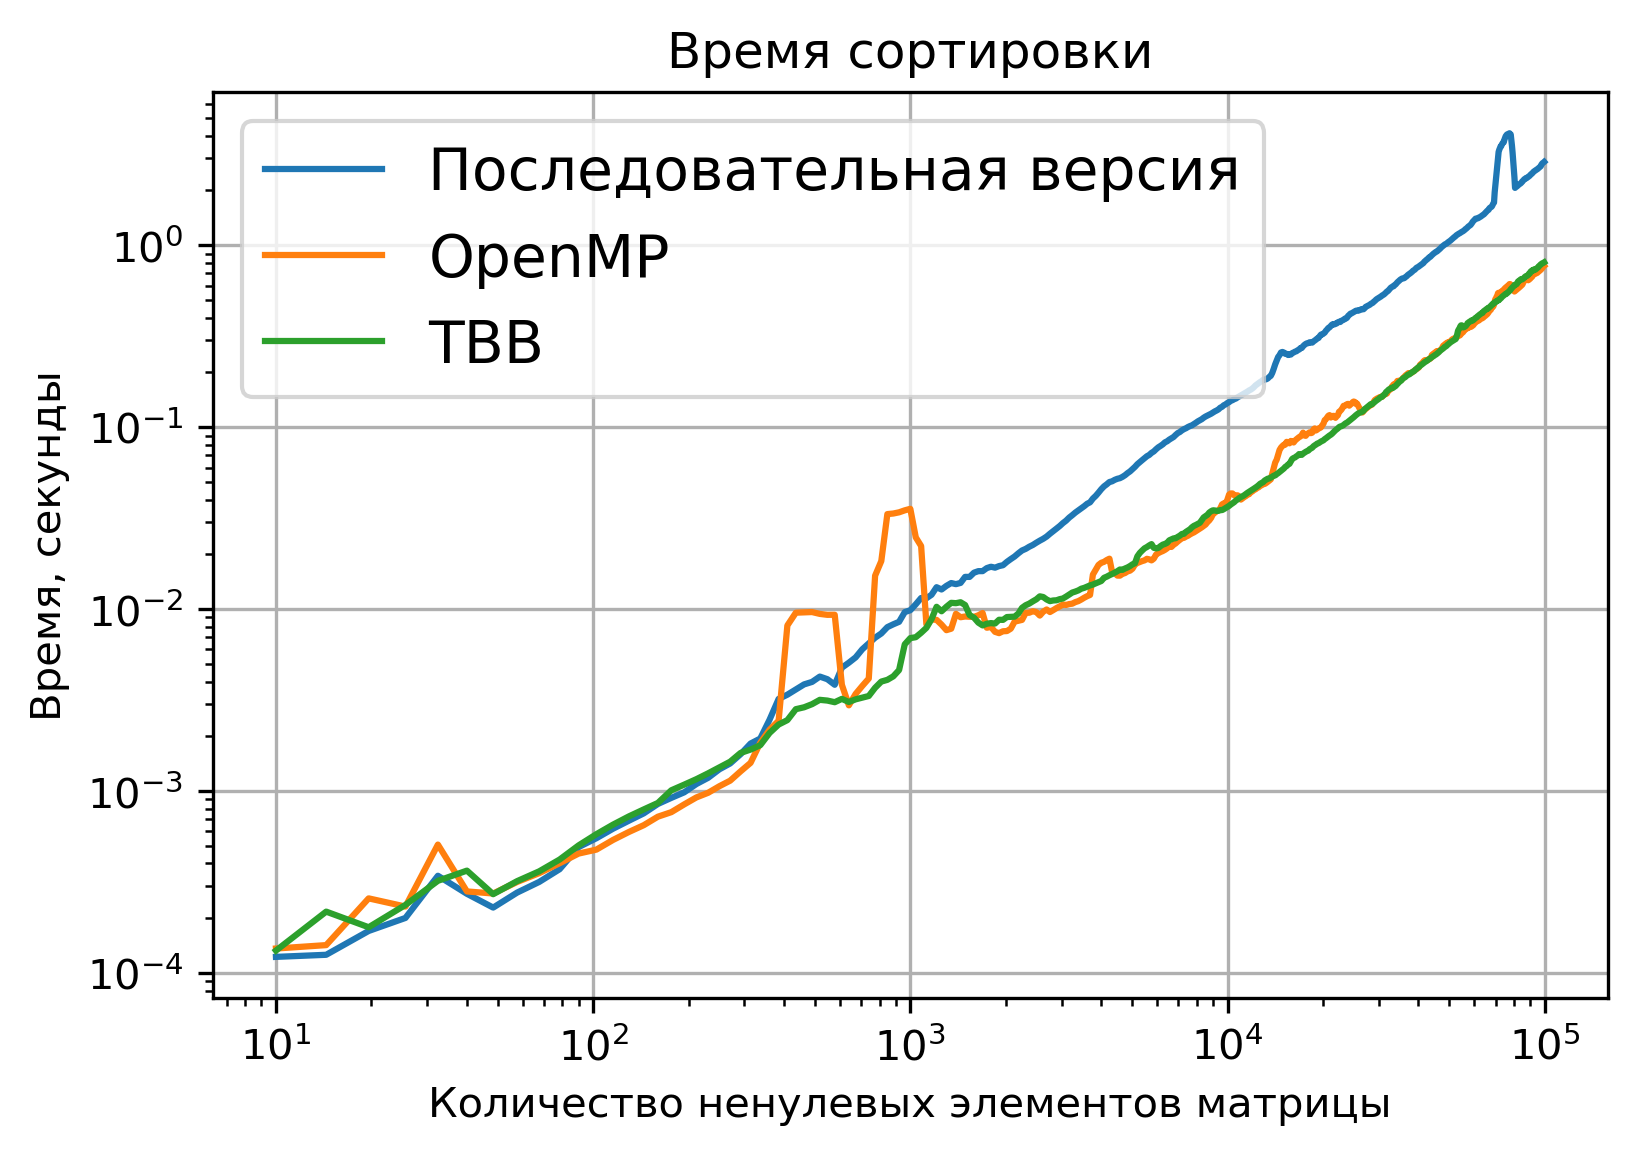
\includegraphics[width=0.85\textwidth]{../../modules/task_1/kolosova_a_complex_ccs/images/time_comparison.png}
    \caption{Сравнение ускорения реализаций сортировок}
    \label{fig:my_label_1}
\end{figure}
\par Был проведен эксперимент по измерению ускорения параллельных версий относительно последовательной с различным размером матриц со средним количеством ненулевых элементов, равным 10\% от общего числа. Для параллельных версий алгоритм выполнялся на 8 потоках. Ось абсцисс показывает количество ненулевых элементов в матрице. Ось ординат показывает, во сколько раз параллельная версия быстрее последовательной на матрицах того же размера, усредненное методом скользящего среднего с окном размера 7.
\begin{figure}[H]
    \centering
    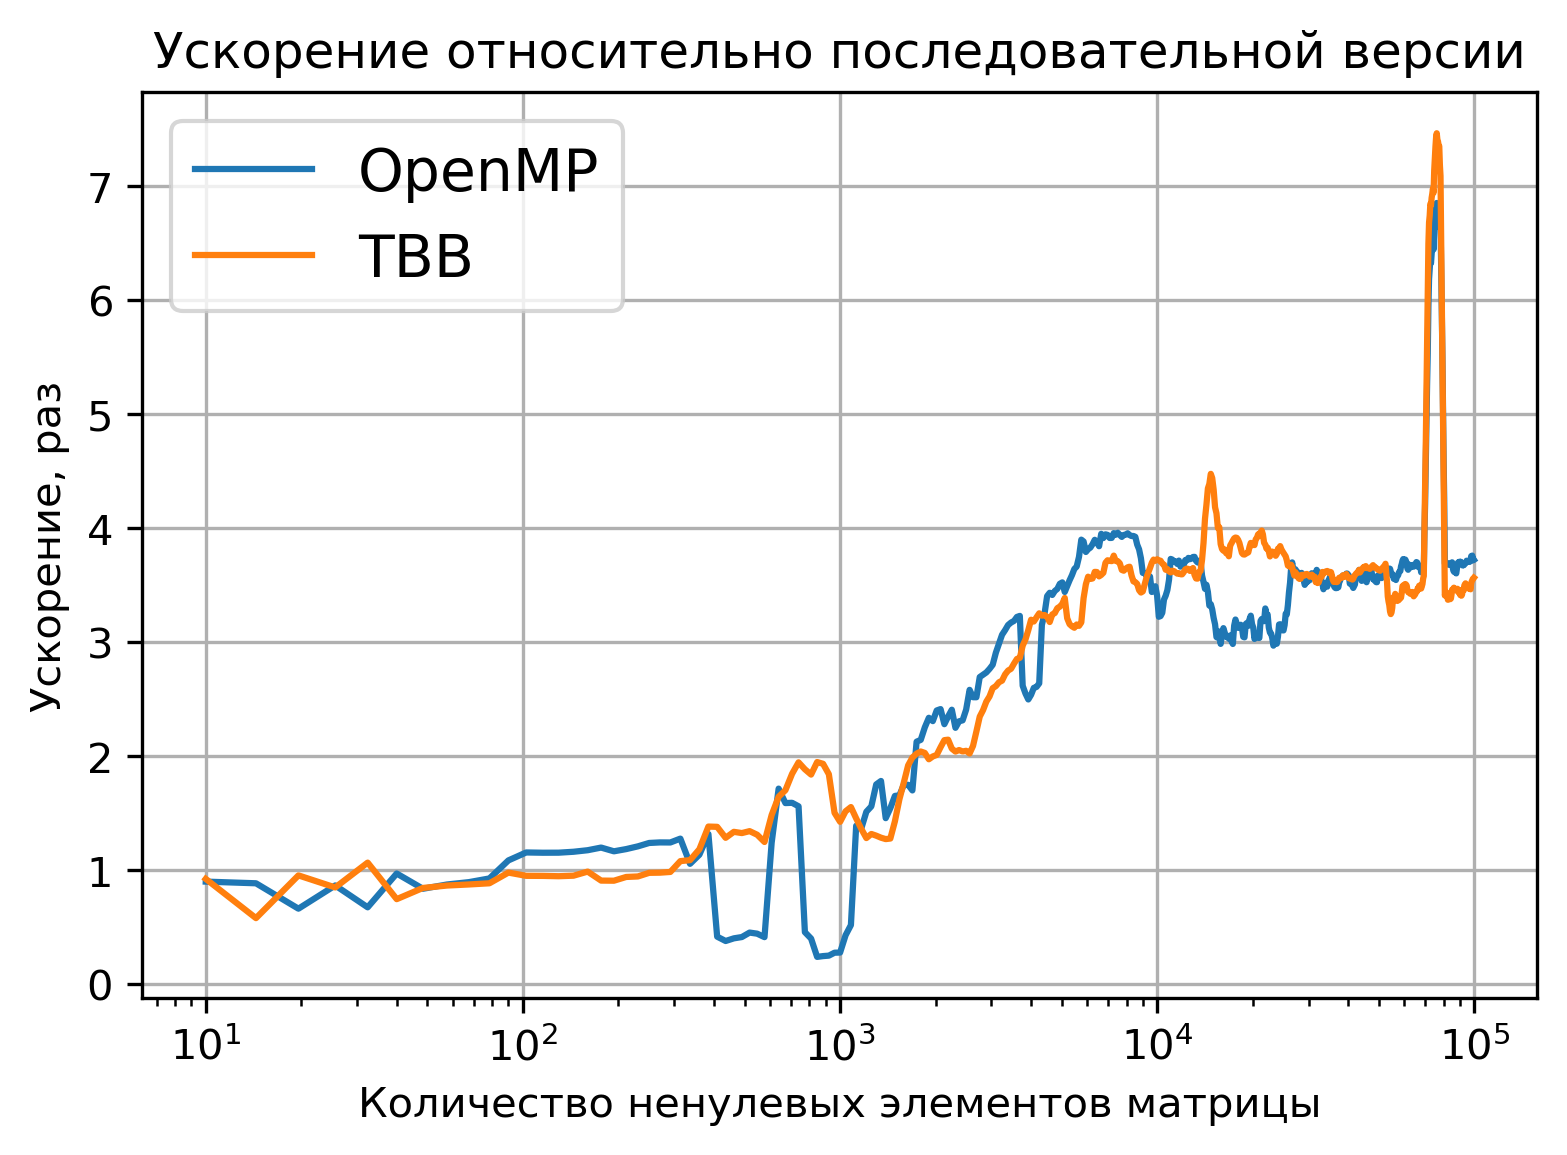
\includegraphics[width=0.85\textwidth]{../../modules/task_1/kolosova_a_complex_ccs/images/speed_comparison.png}
    \caption{Сравнение ускорения реализаций сортировок}
    \label{fig:my_label_1}
\end{figure}

\newpage

% Выводы из результатов экспериментов
\section*{Выводы из результатов экспериментов}
\addcontentsline{toc}{section}{Выводы из результатов экспериментов}
\par Из результатов экспериментов можно сделать следующие выводы:
\begin{itemize}
    \item При увеличении размера матриц увеличивается и эффективность параллельной реализации, т.к. временные затраты на распараллеливание становятся все меньше относительно времени непосредственно выполнения алгоритма, если увеличивается количество обрабатываемых данных.
    \item Параллельные версии начинают давать стабильное преимущество по скорости в 2 раза, начиная примерно с размера матриц 105×105 (около 1100 ненулевых элементов).
    \item Данные реализации на OpenMP и TBB слабо отличаются по эффективности, т.к. были использованы одни из простейших возможных способов распараллеливания. Если бы возможности этих технологий были использованы более широко, возможно, результаты бы более существенно отличались.
\end{itemize}

\newpage

% Заключение
\section*{Заключение}
\addcontentsline{toc}{section}{Заключение}
\par В ходе выполнения лабораторных работ были реализованы последовательная, OpenMP и TBB версии алгоритма умножения разреженных матриц со столбцовым способом хранения, была доказана их корректность работы и проведены эксперименты по определению их эффективности, по результатам которых можно сказать, что с помощью параллельных реализаций алгоритма можно получить значительный прирост скорости, если размер матриц достаточно большой.

\newpage

% Литература
\section*{Литература}
\addcontentsline{toc}{section}{Литература}
\begin{enumerate}
    \item НОУ ИНТУИТ. Лекция 7: Умножение разреженных матриц - Электронный ресурс. URL: \newline
    \url{https://intuit.ru/studies/courses/4447/983/lecture/14931?page=5}
    \item Сысоев А.В. Параллельное программирование с использованием OpenMP. URL: \newline
    \url{https://cloud.unn.ru/s/RQMgkKLMq92cm6A}
    \item Мееров И.Б., Сысоев А.В., Сиднев А.А. Инструменты параллельного программирования для систем с общей памятью. Библиотека Intel Threading Building Blocks. URL: \newline
    \url{https://cloud.unn.ru/s/nS8EtaeH7N4XW7t}
\end{enumerate}
\newpage

% Приложение
\section*{Приложение}
\addcontentsline{toc}{section}{Приложение}
\verb|ccs_complex_mult.h|
\begin{lstlisting}
// Copyright 2022 Kolosova Alena

#ifndef MODULES_TASK_3_KOLOSOVA_A_MULT_COMPLEX_CCS_MATRIX_CCS_COMPLEX_MULT_H_
#define MODULES_TASK_3_KOLOSOVA_A_MULT_COMPLEX_CCS_MATRIX_CCS_COMPLEX_MULT_H_

#include <tbb/tbb.h>
#include <vector>
#include <complex>
#include <iostream>

struct CCS_matrix {
    int row_n;
    int col_n;
    std::vector<std::complex<double>> val;
    std::vector<int> rows;
    std::vector<int> column_pointer;

    friend std::ostream& operator<<(std::ostream& stream, const CCS_matrix& m) {
        stream << "matrix rows = " << m.row_n << " cols = " << m.col_n << std::endl << "values: ";
        for (auto elem : m.val)
            stream << elem << ' ';
        stream << std::endl << "rows: ";
        for (auto elem : m.rows)
            stream << elem << ' ';
        stream << std::endl << "column pointer: ";
        for (auto elem : m.column_pointer)
            stream << elem << ' ';
        stream << std::endl;
        return stream;
    }

    bool operator==(const CCS_matrix& m) const {
        if (m.row_n == row_n && m.col_n == col_n && m.val == val &&
            m.rows == rows && m.column_pointer == column_pointer) return true;
        return false;
    }

    explicit CCS_matrix(int r = 0, int c = 0) {
        row_n = r;
        col_n = c;
    }

    explicit CCS_matrix(std::vector<std::vector<std::complex<double>>> m);
};

std::vector<std::vector<std::complex<double>>> generate_matrix(int r, int c,
    double density = 0.5);

CCS_matrix transpose(const CCS_matrix& A);
CCS_matrix multiply(const CCS_matrix& A, const CCS_matrix& B);

CCS_matrix transpose_tbb(const CCS_matrix& A);
CCS_matrix multiply_tbb(const CCS_matrix& A, const CCS_matrix& B);

std::complex<double> scalar_mult(const std::vector<std::complex<double>>& v1,
    const std::vector<int>& pos1, int start1, int end1,
    const std::vector<std::complex<double>>& v2, const std::vector<int>& pos2,
    int start2, int end2);

#endif  // MODULES_TASK_3_KOLOSOVA_A_MULT_COMPLEX_CCS_MATRIX_CCS_COMPLEX_MULT_H_
\end{lstlisting}
\verb|ccs_complex_mult.cpp| (OpenMP)
\begin{lstlisting}
// Copyright 2022 Kolosova Alena

#include <vector>
#include <random>
#include <iostream>

#include "../../../modules/task_2/kolosova_a_mult_complex_ccs_matrix/ccs_complex_mult.h"

std::vector<std::vector<std::complex<double>>> generate_matrix(int r, int c,
    double density) {
    if (r <= 0 || c <= 0) {
        throw("Incorrect matrix size for generation");
    }
    if (density < 0 || density>1) density = 0.5;

    std::random_device dev;
    std::mt19937 rgen(dev());
    std::uniform_real_distribution<double> prob{ 0.0, 1.0 };
    std::uniform_real_distribution<double> val{ 0.0, 100.0 };
    std::vector<std::vector<std::complex<double>>> matrix(r);

#pragma omp parallel for
    for (int i = 0; i < r; ++i) {
        matrix[i].resize(c);
        for (int j = 0; j < c; ++j) {
            if (prob(rgen) <= density) {
                matrix[i][j] = val(rgen);
            }
        }
    }
    return matrix;
}

CCS_matrix::CCS_matrix(std::vector<std::vector<std::complex<double>>> m) {
    row_n = m.size();
    col_n = (row_n) ? m[0].size() : 0;
    int ptr = 0;
    for (int j = 0; j < col_n; j++) {
        column_pointer.push_back(ptr);
        for (int i = 0; i < row_n; i++) {
            if (m[i][j].real() || m[i][j].imag()) {
                val.push_back(m[i][j]);
                rows.push_back(i);
                ptr++;
            }
        }
    }
    column_pointer.push_back(ptr);
}

CCS_matrix transpose(const CCS_matrix& A) {
    CCS_matrix res(A.col_n, A.row_n);
    std::vector<std::vector<std::complex<double>>> tmpVals(res.col_n);  // vector of new values by columns
    std::vector<std::vector<int>> tmpRows(res.col_n);  // vector of new row indexes

    for (int i = 0; i < A.col_n; i++) {
        for (int j = A.column_pointer[i]; j < A.column_pointer[i + 1]; j++) {
            tmpVals[A.rows[j]].push_back(A.val[j]);
            tmpRows[A.rows[j]].push_back(i);
        }
    }

    int tmpCol = 0;
    for (int i = 0; i < static_cast<int>(tmpVals.size()); i++) {
        res.column_pointer.push_back(tmpCol);
        res.val.insert(res.val.end(), tmpVals[i].begin(), tmpVals[i].end());
        res.rows.insert(res.rows.end(), tmpRows[i].begin(), tmpRows[i].end());
        tmpCol += tmpVals[i].size();
    }
    res.column_pointer.push_back(tmpCol);
    return res;
}

CCS_matrix transpose_omp(const CCS_matrix& A) {
    CCS_matrix res(A.col_n, A.row_n);
    std::vector<std::vector<std::complex<double>>> tmpVals(res.col_n);  // vector of new values by columns
    std::vector<std::vector<int>> tmpRows(res.col_n);  // vector of new row indexes

    for (int i = 0; i < A.col_n; i++) {
#pragma omp parallel for num_threads(8)
        for (int j = A.column_pointer[i]; j < A.column_pointer[i + 1]; j++) {
            tmpVals[A.rows[j]].push_back(A.val[j]);
            tmpRows[A.rows[j]].push_back(i);
        }
    }

    int tmpCol = 0;
    for (int i = 0; i < static_cast<int>(tmpVals.size()); i++) {
        res.column_pointer.push_back(tmpCol);
        res.val.insert(res.val.end(), tmpVals[i].begin(), tmpVals[i].end());
        res.rows.insert(res.rows.end(), tmpRows[i].begin(), tmpRows[i].end());
        tmpCol += tmpVals[i].size();
    }
    res.column_pointer.push_back(tmpCol);
    return res;
}

CCS_matrix multiply(const CCS_matrix& A, const CCS_matrix& B) {
    if (A.col_n != B.row_n)
        throw("Incompatible matrices size for multiplication");
    CCS_matrix At = transpose(A);

    std::vector<std::vector<std::complex<double>>> tmpVals(B.col_n);
    std::vector<std::vector<int>> tmpRows(B.col_n);

    for (int j = 0; j < B.col_n; j++) {
        if (B.column_pointer[j] == B.column_pointer[j + 1]) continue;
        for (int i = 0; i < A.row_n; i++) {
            if (At.column_pointer[i] == At.column_pointer[i + 1]) continue;
            std::complex<double> v = scalar_mult(At.val, At.rows, At.column_pointer[i],
                At.column_pointer[i + 1],
                B.val, B.rows, B.column_pointer[j], B.column_pointer[j + 1]);
            if (v != 0.0) {
                tmpVals[j].push_back(v);
                tmpRows[j].push_back(i);
            }
        }
    }

    CCS_matrix res(A.row_n, B.col_n);
    int tmpCol = 0;
    for (int i = 0; i < res.col_n; i++) {
        res.column_pointer.push_back(tmpCol);
        res.val.insert(res.val.end(), tmpVals[i].begin(), tmpVals[i].end());
        res.rows.insert(res.rows.end(), tmpRows[i].begin(), tmpRows[i].end());
        tmpCol += tmpVals[i].size();
    }
    res.column_pointer.push_back(tmpCol);
    return res;
}

CCS_matrix multiply_omp(const CCS_matrix& A, const CCS_matrix& B) {
    if (A.col_n != B.row_n)
        throw("Incompatible matrices size for multiplication");
    CCS_matrix At = transpose_omp(A);

    std::vector<std::vector<std::complex<double>>> tmpVals(B.col_n);
    std::vector<std::vector<int>> tmpRows(B.col_n);

#pragma omp parallel for num_threads(8)
    for (int j = 0; j < B.col_n; j++) {
        if (B.column_pointer[j] == B.column_pointer[j + 1]) {
            continue;
        }
        for (int i = 0; i < A.row_n; i++) {
            if (At.column_pointer[i] == At.column_pointer[i + 1]) {
                continue;
            }
            std::complex<double> v = scalar_mult(At.val, At.rows, At.column_pointer[i],
                At.column_pointer[i + 1],
                B.val, B.rows, B.column_pointer[j], B.column_pointer[j + 1]);
            if (v != 0.0) {
                tmpVals[j].push_back(v);
                tmpRows[j].push_back(i);
            }
        }
    }

    CCS_matrix res(A.row_n, B.col_n);
    int tmpCol = 0;
    for (int i = 0; i < res.col_n; i++) {
        res.column_pointer.push_back(tmpCol);
        res.val.insert(res.val.end(), tmpVals[i].begin(), tmpVals[i].end());
        res.rows.insert(res.rows.end(), tmpRows[i].begin(), tmpRows[i].end());
        tmpCol += tmpVals[i].size();
    }
    res.column_pointer.push_back(tmpCol);
    return res;
}

std::complex<double> scalar_mult(const std::vector<std::complex<double>>& v1,
    const std::vector<int>& pos1, int start1, int end1,
    const std::vector<std::complex<double>>& v2, const std::vector<int>& pos2,
    int start2, int end2) {
    std::complex<double> res = { 0, 0 };
    for (int i = start1, j = start2; i < end1 && j < end2;) {
        if (pos1[i] == pos2[j]) {
            res += v1[i] * v2[j];
            i++;
            j++;
        } else {
            if (pos1[i] < pos2[j]) i++;
            else
                j++;
        }
    }
    return res;
}

\end{lstlisting}
\verb|main.cpp| (OpenMP)
\begin{lstlisting}
// Copyright 2022 Kolosova Alena
#include <gtest/gtest.h>

#include "./ccs_complex_mult.h"

TEST(CCSComplexMatrix, can_generate_matrix_with_default_density) {
    ASSERT_NO_THROW(generate_matrix(10, 10));
}

TEST(CCSComplexMatrix, can_generate_matrix_with_set_density) {
    ASSERT_NO_THROW(generate_matrix(10, 10, 0.3));
}

TEST(CCSComplexMatrix, can_convert_matrix_to_CCS) {
    std::vector<std::complex<double>> v1{ {0.0, 0.0}, {3.0, 0.0}, {0.0, 0.0}, {0.0, 7.0} };
    std::vector<std::complex<double>> v2{ {0.0, 0.0}, {0.0, 0.0}, {8.0, 0.0}, {0.0, 0.0} };
    std::vector<std::complex<double>> v3{ {0.0, 0.0}, {0.0, 0.0}, {0.0, 0.0}, {0.0, 0.0} };
    std::vector<std::complex<double>> v4{ {9.0, 0.0}, {0.0, 0.0}, {0.0, 15.0}, {0.0, 17.0} };
    std::vector<std::vector<std::complex<double>>> vControl{ v1, v2, v3, v4 };

    CCS_matrix vTest(4, 4);
    vTest.val = { {9.0, 0.0}, {3.0, 0.0}, {8.0, 0.0}, {0.0, 15.0}, {0.0, 7.0}, {0.0, 17.0} };
    vTest.rows = { 3, 0, 1, 3, 0, 3 };
    vTest.column_pointer = { 0, 1, 2, 4, 6 };

    CCS_matrix m(vControl);
    EXPECT_EQ(m, vTest);
}

TEST(CCSComplexMatrix, can_transpose_matrix) {
    std::vector<std::complex<double>> v1{ {0.0, 0.0}, {3.0, 0.0}, {0.0, 0.0}, {0.0, 7.0}, {0.0, 0.0} };
    std::vector<std::complex<double>> v2{ {0.0, 0.0}, {0.0, 0.0}, {8.0, 0.0}, {0.0, 0.0}, {0.0, 0.0} };
    std::vector<std::complex<double>> v3{ {0.0, 0.0}, {0.0, 0.0}, {0.0, 0.0}, {0.0, 0.0}, {0.0, 0.0} };
    std::vector<std::complex<double>> v4{ {9.0, 0.0}, {0.0, 0.0}, {0.0, 15.0}, {0.0, 17.0}, {0.0, 5.0} };
    std::vector<std::vector<std::complex<double>>> m01{ v1, v2, v3, v4 };
    CCS_matrix m1(m01);

    std::vector<std::complex<double>> v11{ {0, 0}, {0, 0}, {0, 0}, {9, 0} };
    std::vector<std::complex<double>> v12{ {3, 0}, {0, 0}, {0, 0}, {0, 0} };
    std::vector<std::complex<double>> v13{ {0, 0}, {8, 0}, {0, 0}, {0, 15} };
    std::vector<std::complex<double>> v14{ {0, 7}, {0, 0}, {0, 0}, {0, 17} };
    std::vector<std::complex<double>> v15{ {0, 0}, {0, 0}, {0, 0}, {0, 5} };
    std::vector<std::vector<std::complex<double>>> m02{ v11, v12, v13, v14, v15 };
    CCS_matrix m2(m02);

    CCS_matrix m2t = transpose(m2);

    EXPECT_EQ(m1, m2t);
}

TEST(CCSComplexMatrix, can_transpose_matrix_omp) {
    CCS_matrix m1(4, 5);
    m1.val = { {9.0, 0.0}, {3.0, 0.0}, {8.0, 0.0}, {0.0, 15.0}, {0.0, 7.0}, {0.0, 17.0}, {0.0, 5.0} };
    m1.rows = { 3, 0, 1, 3, 0, 3 , 3 };
    m1.column_pointer = { 0, 1, 2, 4, 6, 7 };

    CCS_matrix m2(5, 4);
    m2.val = { {3.0, 0.0}, {0.0, 7.0}, {8.0, 0.0}, {9.0, 0.0}, {0.0, 15.0}, {0.0, 17.0}, {0.0, 5.0} };
    m2.rows = { 1, 3, 2, 0, 2, 3, 4 };
    m2.column_pointer = { 0, 2, 3, 3, 7 };

    CCS_matrix m2t = transpose_omp(m2);

    EXPECT_EQ(m1, m2t);
}

TEST(CCSComplexMatrix, throws_when_CCS_matrices_are_of_incompatible_size) {
    CCS_matrix m1(2, 3), m2(4, 5);
    EXPECT_ANY_THROW(multiply(m1, m2));
}

TEST(CCSComplexMatrix, throws_when_CCS_matrices_are_of_incompatible_size_omp) {
    CCS_matrix m1(2, 3), m2(4, 5);
    EXPECT_ANY_THROW(multiply_omp(m1, m2));
}

TEST(CCSComplexMatrix, can_multiply_small_CCS_matrices) {
    double t1, t2, dt;

    std::vector<std::vector<std::complex<double>>> tmp1 = generate_matrix(10, 10, 0.1),
        tmp2 = generate_matrix(10, 10, 0.1);
    CCS_matrix m1(tmp1), m2(tmp2);

    t1 = omp_get_wtime();
    CCS_matrix res1 = multiply(m1, m2);
    t2 = omp_get_wtime();
    dt = t2 - t1;
    std::cerr << "Sequential: " << dt << std::endl;

    t1 = omp_get_wtime();
    CCS_matrix res2 = multiply_omp(m1, m2);
    t2 = omp_get_wtime();
    dt = t2 - t1;
    std::cerr << "Parallel: " << dt << std::endl;

    EXPECT_EQ(res1, res2);
}

TEST(CCSComplexMatrix, can_multiply_medium_CCS_matrices) {
    double t1, t2, dt;

    std::vector<std::vector<std::complex<double>>> tmp1 = generate_matrix(100, 100, 0.1),
        tmp2 = generate_matrix(100, 100, 0.1);
    CCS_matrix m1(tmp1), m2(tmp2);

    t1 = omp_get_wtime();
    CCS_matrix res1 = multiply(m1, m2);
    t2 = omp_get_wtime();
    dt = t2 - t1;
    std::cerr << "Sequential: " << dt << std::endl;

    t1 = omp_get_wtime();
    CCS_matrix res2 = multiply_omp(m1, m2);
    t2 = omp_get_wtime();
    dt = t2 - t1;
    std::cerr << "Parallel: " << dt << std::endl;

    EXPECT_EQ(res1, res2);
}

TEST(CCSComplexMatrix, can_multiply_large_CCS_matrices) {
    double t1, t2, dt;

    std::vector<std::vector<std::complex<double>>> tmp1 = generate_matrix(1000, 1000, 0.1),
        tmp2 = generate_matrix(1000, 1000, 0.1);
    CCS_matrix m1(tmp1), m2(tmp2);

    t1 = omp_get_wtime();
    CCS_matrix res1 = multiply(m1, m2);
    t2 = omp_get_wtime();
    dt = t2 - t1;
    std::cerr << "Sequential: " << dt << std::endl;

    t1 = omp_get_wtime();
    CCS_matrix res2 = multiply_omp(m1, m2);
    t2 = omp_get_wtime();
    dt = t2 - t1;
    std::cerr << "Parallel: " << dt << std::endl;

    EXPECT_EQ(res1, res2);
}

int main(int argc, char **argv) {
    ::testing::InitGoogleTest(&argc, argv);
    return RUN_ALL_TESTS();
}
\end{lstlisting}
\verb|ccs_complex_mult.cpp| (TBB)
\begin{lstlisting}
// Copyright 2022 Kolosova Alena

#include <vector>
#include <random>
#include <iostream>

#include "../../../modules/task_3/kolosova_a_mult_complex_ccs_matrix/ccs_complex_mult.h"

std::vector<std::vector<std::complex<double>>> generate_matrix(int r, int c,
    double density) {
    if (r <= 0 || c <= 0) {
        throw("Incorrect matrix size for generation");
    }
    if (density < 0 || density > 1) density = 0.5;

    std::random_device dev;
    std::mt19937 rgen(dev());
    std::uniform_real_distribution<double> prob{ 0.0, 1.0 };
    std::uniform_real_distribution<double> val{ 0.0, 100.0 };
    std::vector<std::vector<std::complex<double>>> matrix(r);

    for (int i = 0; i < r; ++i) {
        matrix[i].resize(c);
        tbb::parallel_for(tbb::blocked_range<size_t>(0, c),
            [&](const tbb::blocked_range<size_t>& range) {
                int begin = range.begin(), end = range.end();
                for (int j = begin; j < end; j++) {
                    if (prob(rgen) <= density) {
                        matrix[i][j] = val(rgen);
                    }
                }
            });
    }
    return matrix;
}

CCS_matrix::CCS_matrix(std::vector<std::vector<std::complex<double>>> m) {
    row_n = m.size();
    col_n = (row_n) ? m[0].size() : 0;
    int ptr = 0;
    for (int j = 0; j < col_n; j++) {
        column_pointer.push_back(ptr);
        for (int i = 0; i < row_n; i++) {
            if (m[i][j].real() || m[i][j].imag()) {
                val.push_back(m[i][j]);
                rows.push_back(i);
                ptr++;
            }
        }
    }
    column_pointer.push_back(ptr);
}

CCS_matrix transpose(const CCS_matrix& A) {
    CCS_matrix res(A.col_n, A.row_n);
    std::vector<std::vector<std::complex<double>>> tmpVals(res.col_n);  // vector of new values by columns
    std::vector<std::vector<int>> tmpRows(res.col_n);  // vector of new row indexes

    for (int i = 0; i < A.col_n; i++) {
        for (int j = A.column_pointer[i]; j < A.column_pointer[i + 1]; j++) {
            tmpVals[A.rows[j]].push_back(A.val[j]);
            tmpRows[A.rows[j]].push_back(i);
        }
    }

    int tmpCol = 0;
    for (int i = 0; i < static_cast<int>(tmpVals.size()); i++) {
        res.column_pointer.push_back(tmpCol);
        res.val.insert(res.val.end(), tmpVals[i].begin(), tmpVals[i].end());
        res.rows.insert(res.rows.end(), tmpRows[i].begin(), tmpRows[i].end());
        tmpCol += tmpVals[i].size();
    }
    res.column_pointer.push_back(tmpCol);
    return res;
}

CCS_matrix transpose_tbb(const CCS_matrix& A) {
    CCS_matrix res(A.col_n, A.row_n);
    std::vector<std::vector<std::complex<double>>> tmpVals(res.col_n);  // vector of new values by columns
    std::vector<std::vector<int>> tmpRows(res.col_n);  // vector of new row indexes

    for (int i = 0; i < A.col_n; i++) {
        tbb::parallel_for(tbb::blocked_range<size_t>(A.column_pointer[i], A.column_pointer[i + 1]),
            [&](const tbb::blocked_range<size_t>& r) {
                int begin = r.begin(), end = r.end();
                for (int j = begin; j < end; j++) {
                    tmpVals[A.rows[j]].push_back(A.val[j]);
                    tmpRows[A.rows[j]].push_back(i);
                }
            });
    }

    int tmpCol = 0;
    for (int i = 0; i < static_cast<int>(tmpVals.size()); i++) {
        res.column_pointer.push_back(tmpCol);
        res.val.insert(res.val.end(), tmpVals[i].begin(), tmpVals[i].end());
        res.rows.insert(res.rows.end(), tmpRows[i].begin(), tmpRows[i].end());
        tmpCol += tmpVals[i].size();
    }
    res.column_pointer.push_back(tmpCol);
    return res;
}

CCS_matrix multiply(const CCS_matrix& A, const CCS_matrix& B) {
    if (A.col_n != B.row_n)
        throw("Incompatible matrices size for multiplication");
    CCS_matrix At = transpose(A);

    std::vector<std::vector<std::complex<double>>> tmpVals(B.col_n);
    std::vector<std::vector<int>> tmpRows(B.col_n);

    for (int j = 0; j < B.col_n; j++) {
        if (B.column_pointer[j] == B.column_pointer[j + 1]) continue;
        for (int i = 0; i < A.row_n; i++) {
            if (At.column_pointer[i] == At.column_pointer[i + 1]) continue;
            std::complex<double> v = scalar_mult(At.val, At.rows, At.column_pointer[i],
                At.column_pointer[i + 1],
                B.val, B.rows, B.column_pointer[j], B.column_pointer[j + 1]);
            if (v != 0.0) {
                tmpVals[j].push_back(v);
                tmpRows[j].push_back(i);
            }
        }
    }

    CCS_matrix res(A.row_n, B.col_n);
    int tmpCol = 0;
    for (int i = 0; i < res.col_n; i++) {
        res.column_pointer.push_back(tmpCol);
        res.val.insert(res.val.end(), tmpVals[i].begin(), tmpVals[i].end());
        res.rows.insert(res.rows.end(), tmpRows[i].begin(), tmpRows[i].end());
        tmpCol += tmpVals[i].size();
    }
    res.column_pointer.push_back(tmpCol);
    return res;
}

CCS_matrix multiply_tbb(const CCS_matrix& A, const CCS_matrix& B) {
    if (A.col_n != B.row_n)
        throw("Incompatible matrices size for multiplication.");
    CCS_matrix At = transpose_tbb(A);

    std::vector<std::vector<std::complex<double>>> tmpVals(B.col_n);
    std::vector<std::vector<int>> tmpRows(B.col_n);

    tbb::parallel_for(tbb::blocked_range<size_t>(0, B.col_n),
        [&](const tbb::blocked_range<size_t>& r) {
            int begin = r.begin(), end = r.end();
            for (int j = begin; j < end; j++) {
                if (B.column_pointer[j] == B.column_pointer[j + 1]) {
                    continue;
                }
                for (int i = 0; i < A.row_n; i++) {
                    if (At.column_pointer[i] == At.column_pointer[i + 1]) {
                        continue;
                    }
                    std::complex<double> v = scalar_mult(At.val, At.rows, At.column_pointer[i],
                        At.column_pointer[i + 1],
                        B.val, B.rows, B.column_pointer[j], B.column_pointer[j + 1]);
                    if (v != 0.0) {
                        tmpVals[j].push_back(v);
                        tmpRows[j].push_back(i);
                    }
                }
            }
        });

    CCS_matrix res(A.row_n, B.col_n);
    int tmpCol = 0;
    for (int i = 0; i < res.col_n; i++) {
        res.column_pointer.push_back(tmpCol);
        res.val.insert(res.val.end(), tmpVals[i].begin(), tmpVals[i].end());
        res.rows.insert(res.rows.end(), tmpRows[i].begin(), tmpRows[i].end());
        tmpCol += tmpVals[i].size();
    }
    res.column_pointer.push_back(tmpCol);
    return res;
}

std::complex<double> scalar_mult(const std::vector<std::complex<double>>& v1,
    const std::vector<int>& pos1, int start1, int end1,
    const std::vector<std::complex<double>>& v2, const std::vector<int>& pos2,
    int start2, int end2) {
    std::complex<double> res = { 0, 0 };
    for (int i = start1, j = start2; i < end1 && j < end2;) {
        if (pos1[i] == pos2[j]) {
            res += v1[i] * v2[j];
            i++;
            j++;
        } else {
            if (pos1[i] < pos2[j]) i++;
            else
                j++;
        }
    }
    return res;
}

\end{lstlisting}
\verb|main.cpp| (TBB)
\begin{lstlisting}
// Copyright 2022 Kolosova Alena
#include <gtest/gtest.h>

#include "./ccs_complex_mult.h"

TEST(CCSComplexMatrix, can_generate_matrix_with_default_density) {
    ASSERT_NO_THROW(generate_matrix(10, 10));
}

TEST(CCSComplexMatrix, can_generate_matrix_with_set_density) {
    ASSERT_NO_THROW(generate_matrix(10, 10, 0.3));
}

TEST(CCSComplexMatrix, can_convert_matrix_to_CCS) {
    std::vector<std::complex<double>> v1{ {0.0, 0.0}, {3.0, 0.0}, {0.0, 0.0}, {0.0, 7.0} };
    std::vector<std::complex<double>> v2{ {0.0, 0.0}, {0.0, 0.0}, {8.0, 0.0}, {0.0, 0.0} };
    std::vector<std::complex<double>> v3{ {0.0, 0.0}, {0.0, 0.0}, {0.0, 0.0}, {0.0, 0.0} };
    std::vector<std::complex<double>> v4{ {9.0, 0.0}, {0.0, 0.0}, {0.0, 15.0}, {0.0, 17.0} };
    std::vector<std::vector<std::complex<double>>> vControl{ v1, v2, v3, v4 };

    CCS_matrix vTest(4, 4);
    vTest.val = { {9.0, 0.0}, {3.0, 0.0}, {8.0, 0.0}, {0.0, 15.0}, {0.0, 7.0}, {0.0, 17.0} };
    vTest.rows = { 3, 0, 1, 3, 0, 3 };
    vTest.column_pointer = { 0, 1, 2, 4, 6 };

    CCS_matrix m(vControl);
    EXPECT_EQ(m, vTest);
}

TEST(CCSComplexMatrix, can_transpose_matrix) {
    std::vector<std::complex<double>> v1{ {0.0, 0.0}, {3.0, 0.0}, {0.0, 0.0}, {0.0, 7.0}, {0.0, 0.0} };
    std::vector<std::complex<double>> v2{ {0.0, 0.0}, {0.0, 0.0}, {8.0, 0.0}, {0.0, 0.0}, {0.0, 0.0} };
    std::vector<std::complex<double>> v3{ {0.0, 0.0}, {0.0, 0.0}, {0.0, 0.0}, {0.0, 0.0}, {0.0, 0.0} };
    std::vector<std::complex<double>> v4{ {9.0, 0.0}, {0.0, 0.0}, {0.0, 15.0}, {0.0, 17.0}, {0.0, 5.0} };
    std::vector<std::vector<std::complex<double>>> m01{ v1, v2, v3, v4 };
    CCS_matrix m1(m01);

    std::vector<std::complex<double>> v11{ {0, 0}, {0, 0}, {0, 0}, {9, 0} };
    std::vector<std::complex<double>> v12{ {3, 0}, {0, 0}, {0, 0}, {0, 0} };
    std::vector<std::complex<double>> v13{ {0, 0}, {8, 0}, {0, 0}, {0, 15} };
    std::vector<std::complex<double>> v14{ {0, 7}, {0, 0}, {0, 0}, {0, 17} };
    std::vector<std::complex<double>> v15{ {0, 0}, {0, 0}, {0, 0}, {0, 5} };
    std::vector<std::vector<std::complex<double>>> m02{ v11, v12, v13, v14, v15 };
    CCS_matrix m2(m02);

    CCS_matrix m2t = transpose(m2);

    EXPECT_EQ(m1, m2t);
}

TEST(CCSComplexMatrix, can_transpose_matrix_tbb) {
    CCS_matrix m1(4, 5);
    m1.val = { {9.0, 0.0}, {3.0, 0.0}, {8.0, 0.0}, {0.0, 15.0}, {0.0, 7.0}, {0.0, 17.0}, {0.0, 5.0} };
    m1.rows = { 3, 0, 1, 3, 0, 3 , 3 };
    m1.column_pointer = { 0, 1, 2, 4, 6, 7 };

    CCS_matrix m2(5, 4);
    m2.val = { {3.0, 0.0}, {0.0, 7.0}, {8.0, 0.0}, {9.0, 0.0}, {0.0, 15.0}, {0.0, 17.0}, {0.0, 5.0} };
    m2.rows = { 1, 3, 2, 0, 2, 3, 4 };
    m2.column_pointer = { 0, 2, 3, 3, 7 };

    CCS_matrix m2t = transpose_tbb(m2);

    EXPECT_EQ(m1, m2t);
}

TEST(CCSComplexMatrix, throws_when_CCS_matrices_are_of_incompatible_size) {
    CCS_matrix m1(2, 3), m2(4, 5);
    EXPECT_ANY_THROW(multiply(m1, m2));
}

TEST(CCSComplexMatrix, throws_when_CCS_matrices_are_of_incompatible_size_tbb) {
    CCS_matrix m1(2, 3), m2(4, 5);
    EXPECT_ANY_THROW(multiply_tbb(m1, m2));
}

TEST(CCSComplexMatrix, can_multiply_small_CCS_matrices) {
    std::vector<std::vector<std::complex<double>>> tmp1 = generate_matrix(10, 10, 0.1),
        tmp2 = generate_matrix(10, 10, 0.1);
    CCS_matrix m1(tmp1), m2(tmp2);

    tbb::tick_count start1 = tbb::tick_count::now();
    CCS_matrix res1 = multiply(m1, m2);
    tbb::tick_count end1 = tbb::tick_count::now();
    double dt1 = (end1 - start1).seconds();
    std::cerr << "Sequential: " << dt1 << std::endl;

    tbb::tick_count start2 = tbb::tick_count::now();
    CCS_matrix res2 = multiply_tbb(m1, m2);
    tbb::tick_count end2 = tbb::tick_count::now();
    double dt2 = (end2 - start2).seconds();
    std::cerr << "Parallel: " << dt2 << std::endl;

    EXPECT_EQ(res1, res2);
}

TEST(CCSComplexMatrix, can_multiply_medium_CCS_matrices) {
    std::vector<std::vector<std::complex<double>>> tmp1 = generate_matrix(100, 100, 0.1),
        tmp2 = generate_matrix(100, 100, 0.1);
    CCS_matrix m1(tmp1), m2(tmp2);

    tbb::tick_count start1 = tbb::tick_count::now();
    CCS_matrix res1 = multiply(m1, m2);
    tbb::tick_count end1 = tbb::tick_count::now();
    double dt1 = (end1 - start1).seconds();
    std::cerr << "Sequential: " << dt1 << std::endl;

    tbb::tick_count start2 = tbb::tick_count::now();
    CCS_matrix res2 = multiply_tbb(m1, m2);
    tbb::tick_count end2 = tbb::tick_count::now();
    double dt2 = (end2 - start2).seconds();
    std::cerr << "Parallel: " << dt2 << std::endl;

    EXPECT_EQ(res1, res2);
}

TEST(CCSComplexMatrix, can_multiply_large_CCS_matrices) {
    std::vector<std::vector<std::complex<double>>> tmp1 = generate_matrix(1000, 1000, 0.1),
        tmp2 = generate_matrix(1000, 1000, 0.1);
    CCS_matrix m1(tmp1), m2(tmp2);

    tbb::tick_count start1 = tbb::tick_count::now();
    CCS_matrix res1 = multiply(m1, m2);
    tbb::tick_count end1 = tbb::tick_count::now();
    double dt1 = (end1 - start1).seconds();
    std::cerr << "Sequential: " << dt1 << std::endl;

    tbb::tick_count start2 = tbb::tick_count::now();
    CCS_matrix res2 = multiply_tbb(m1, m2);
    tbb::tick_count end2 = tbb::tick_count::now();
    double dt2 = (end2 - start2).seconds();
    std::cerr << "Parallel: " << dt2 << std::endl;

    EXPECT_EQ(res1, res2);
}

int main(int argc, char **argv) {
    ::testing::InitGoogleTest(&argc, argv);
    return RUN_ALL_TESTS();
}
\end{lstlisting}
\end{document}